\documentclass[a4paper, 11pt]{article}

\usepackage[portuges]{babel}
\usepackage[utf8]{inputenc}
\usepackage{amsmath}
\usepackage{indentfirst}
\usepackage[table,xcdraw]{xcolor}
\usepackage{graphicx}
\usepackage{tabto}
\usepackage{float}
\usepackage{adjustbox}
\usepackage[pdftex]{color,graphicx}
\usepackage[left=2cm,top=2.5cm,right=2.5cm,bottom=2.5cm]{geometry}
\usepackage{enumerate}% http://ctan.org/pkg/enumerate
\usepackage{xurl}
\usepackage{hyperref}

\begin{document}
\begin{titlepage}
    \begin{center}

    	
\includegraphics[width=0.3\textwidth]{images/Capa/EEUMfinal .png}
       
       \vspace*{1cm}
       
       \textbf{\Large Engenharia de Serviços em Rede}
        \vspace{1cm}
        \par
        \textbf{\Large Streaming de áudio e vídeo a pedido e em tempo real }
        \vspace{1cm}
        \par
        \Large \textbf{PL3 - Grupo 5}
        
       Luis Sousa a89597\\Maria Barros pg47488\\Pedro Barbosa pg47577
       \vspace{1cm}
	\begin{figure}[!htb]
	    \hspace{1.5cm}
        \minipage{0.25\textwidth}%
            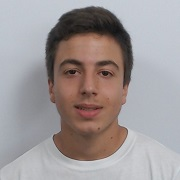
\includegraphics[width=\linewidth]{images/Capa/80.jpg} 
            \centering
            \captionsetup{a89597}
        \endminipage
        \hspace{-0.2cm}
        \minipage{0.25\textwidth}%
            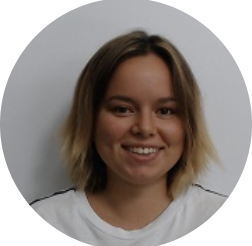
\includegraphics[width=\linewidth]{images/Capa/44.jpg} 
            \centering
            \captionsetup{pg47488}
        \endminipage
        \hspace{-0.2cm}
        \minipage{0.25\textwidth}%
            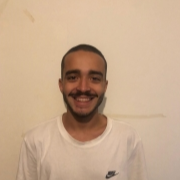
\includegraphics[width=\linewidth]{images/Capa/154.jpg} 
            \centering
            \captionsetup{pg47577}
        \endminipage
    \end{figure}

\blindtext

\vspace{2cm}
        
        16 de novembro de 2021
            
    \end{center}
\end{titlepage}

\newpage
\tableofcontents
\newpage

%----------------------------- Q1 -----------------------------%
\section {Questão 1} 
\textbf{Capture três pequenas amostras de trágefo no link de saída do servidor, respetivamente com 1 cliente (VLC), com 2
clientes (VLC e Firefox) e com 3 clientes (VLC, Firefox e ffmeg). Identifique a taxa em bps necessária (usando o ffmpeg -i video1.mp4
e/ou o próprio wireshark), o encapsulamento usado e o número total de fluxos gerados. Comente a escalabilidade da solução.
Ilustre com evidências da realização prática do exercício (ex: capturas de ecrã)}
\vspace{0.25cm}

Correndo o comando "ffmpeg -i video1.mp4 -hide\_banner" obtemos informação relativa ao ficheiro "video1.mp4". Observando o \textit{output} do comando, concluímos que a taxa em bps necessária (ou \textit{bitrate}) é de 8 kb/s.

\begin{figure}[H]
    \centering
    \frame{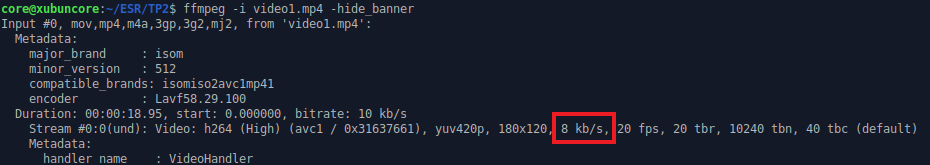
\includegraphics[width=.9\textwidth]{images/q1/bitrate_video1.png}}
    \caption{Detalhes video1.mp4}
\end{figure}

Os 3 clientes de streaming usados neste exercício (VLC, Firefox e ffmpeg) usam HTTP Streaming. Desta forma os clientes estabelecem uma conexão TCP com o servidor que contém o vídeo guardado e enviam um pedido HTTP GET para o URL da stream. Depois, todos os pacotes são transmitidos via a conexão estabelecida, logo, o encapsulamento usado é TCP. \cite{livro}

Na figura seguinte podemos ver o estabelecimento da ligação entre o Portátil 1 e o Streamer nos frames 19 a 21, o pedido HTTP GET no frame 22 e a transmissão dos pacotes relativos ao conteúdo do vídeo nos restantes frames.

\begin{figure}[H]
    \centering
    \frame{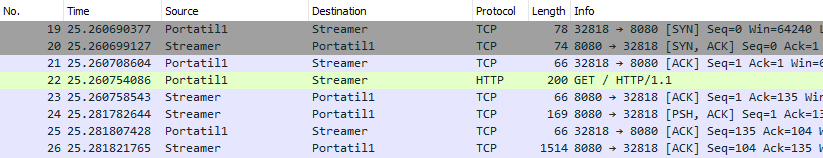
\includegraphics[width=.9\textwidth]{images/q1/inicio transmissao.png}}
    \caption{Início da transmissão do Streamer para o Portátil 1}
\end{figure}

Para o cálculo do total de fluxos gerados no link de saída do servidor, decidimos filtrar os pacotes HTTP GET, pois, no HTTP Streaming, são estes que abrem a porta para o fluxo de pacotes TCP, do streamer para o cliente. Neste cenário, foram gerados 3 fluxos, um para cada portátil conectado à stream.

\begin{figure}[H]
    \centering
    \frame{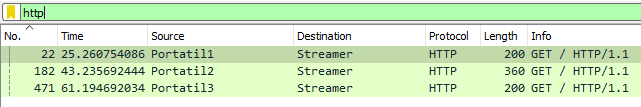
\includegraphics[width=.9\textwidth]{images/q1/fluxos gerados.png}}
    \caption{Pacotes HTTP GET recebidos pelo Streamer}
\end{figure}

De forma a perceber a escalabilidade desta solução de streaming, decidimos analisar o tráfego, com origem no Streamer, para as 3 fases (1 cliente, 2 clientes e 3 clientes).

Assim, usamos o filtro ``ip.src == 10.0.0.10'' para apenas serem apresentados os pacotes com origem no Streamer.

Para analisar o fluxo nas diferentes fases, usamos o filtro ``frame.number $>$= x \&\& frame.number $<$ y'' para captar apenas os pacotes relativos a cada uma delas. Depois, usamos a funcionalidade \textit{Statistics -$>$ Protocol Hierarchy} do Wireshark que nos apresenta informação relativa aos pacotes filtrados, permitindo-nos calcular o tráfego na rede.

Pela análise das três figuras seguintes, mais especificamente da coluna \textit{Bits/s}, podemos observar que o tráfego TCP no link de saída do servidor é 44kbps, 84kbps e 121kbps para 1, 2 e 3 clientes conectados, respetivamente. Desta forma, podemos concluir que a taxa de pacotes enviados pelo servidor tem tendência a aumentar linearmente com o número de clientes conectados, neste caso, cerca de 40kbps por cliente.

\begin{figure}[H]
    \centering
    \frame{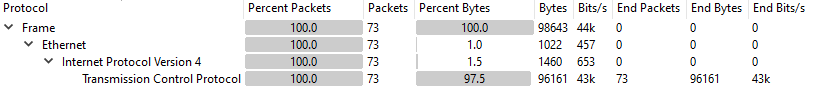
\includegraphics[width=.9\textwidth]{images/q1/fluxo 1 cliente.png}}
    \caption{\textit{Protocol Hierarchy} com 1 cliente}
\end{figure}

\begin{figure}[H]
    \centering
    \frame{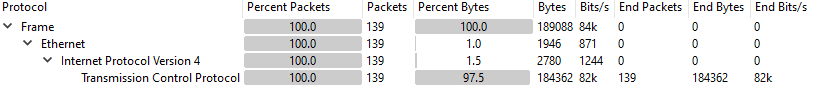
\includegraphics[width=.9\textwidth]{images/q1/fluxo 2 clientes.png}}
    \caption{\textit{Protocol Hierarchy} com 2 clientes}
\end{figure}

\begin{figure}[H]
    \centering
    \frame{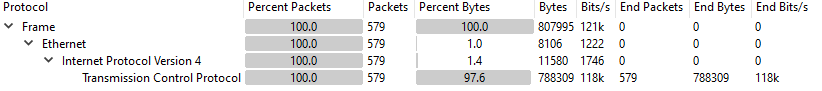
\includegraphics[width=.9\textwidth]{images/q1/fluxo 3 clientes.png}}
    \caption{\textit{Protocol Hierarchy} com 3 clientes}
\end{figure}


%----------------------------- Q2 -----------------------------%
\section{Questão 2}
\textbf{Diga qual a largura de banda necessária, em bits por segundo, para que o cliente de streaming consiga receber o
vídeo no firefox e qual a pilha protocolar usada neste cenário.}
\vspace{0.25cm}

Observando os detalhes do ficheiro "video2.mp4", presentes na figura seguinte, podemos concluir que a largura de banda necessária para que o cliente de streaming consiga receber o vídeo no Firefox é 14 kbps.

\begin{figure}[H]
    \centering
    \frame{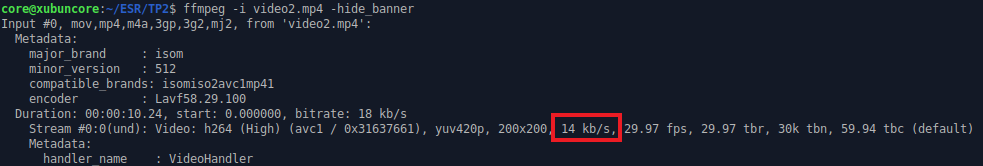
\includegraphics[width=.9\textwidth]{images/q2/bitrate_video2.png}}
    \caption{Detalhes video2.mp4}
\end{figure}

Em relação à pilha protocolar usada neste cenário (TCP/IP), podemos referir os protocolos mais relevantes, para cada uma das camadas.

\begin{itemize}
    \item \textbf{Camada de aplicação:} nesta camada destaca-se o protocolo HTTP, pois é este que é usado para estabelecer a ligação entre o cliente e o servidor, através de um pedido HTTP GET.
    \item \textbf{Camada de transporte:} nesta camada destaca-se o protocolo TCP, maioritariamente usado para a transmissão dos dados do ficheiro em streaming. O pedido HTTP GET também está emcapsulado em TCP.
    \item \textbf{Camada de rede:} nesta camada destaca-se o protocolo IPv4.
    \item \textbf{Camada de ligação:} nesta camada destaca-se o protocolo Ethernet II.
\end{itemize}

Na figura seguinte, podemos ver os diferentes protocolos referidos em cima, num pacote de um pedido HTTP GET.

\begin{figure}[H]
    \centering
    \frame{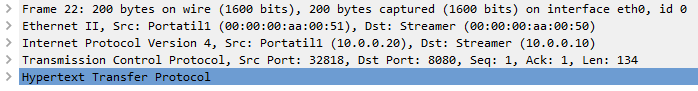
\includegraphics[width=.9\textwidth]{images/q2/frame http get.png}}
    \caption{Frame de um pedido HTTP GET}
\end{figure}


%----------------------------- Q3 -----------------------------%
\section{Questão 3}
\textbf{Ajuste o débito dos links da topologia de modo que o cliente no portátil 2 exiba o vídeo de menor resolução e o cliente
no portátil 1 exiba o vídeo com mais resolução. Mostre evidências.}
\vspace{0.25cm}

Na figura seguinte podemos observar os Portáteis 1 e 2 conectados à stream via DASH, fornecida pelo Streamer. Neste caso, o débito do link para o Portátil 2 foi diminuído, forçando-o a optar pelo vídeo com menor resolução, já o Portátil 1 consegue receber dados a uma taxa que lhe permite apresentar o vídeo de maior resolução.

\begin{figure}[H]
    \centering
    \frame{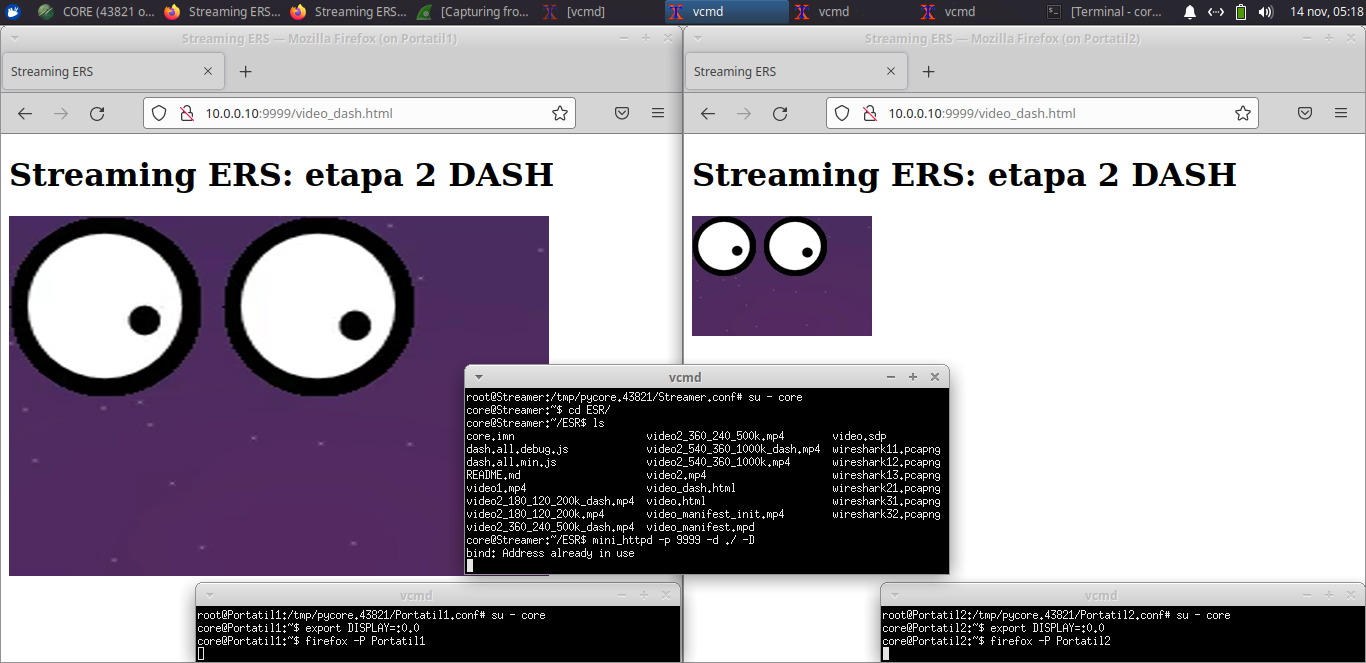
\includegraphics[width=.9\textwidth]{images/q3/streaming debito alterado.png}}
    \caption{Streaming via DASH para dois portáteis}
\end{figure}

\begin{figure}[H]
    \centering
    \frame{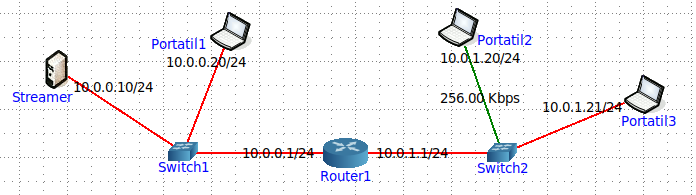
\includegraphics[width=.9\textwidth]{images/q3/topologia debito alterado.png}}
    \caption{Topologia com débito para o Portátil 2 alterado}
\end{figure}

%----------------------------- Q4 -----------------------------%
\section{Questão 4}
\textbf{Descreva o funcionamento do DASH neste caso concreto, referindo o papel do ficheiro MPD criado.}
\vspace{0.25cm}

Para o DASH funcionar corretamente, é necessário criar várias versões do vídeo, com bitrates diferentes (quer seja alterando a sua resolução ou a taxa de frames), atribuindo um URL único para cada uma. Também é preciso criar um ficheiro de manifesto, onde são apresentadas várias informações em relação aos ficheiros de streaming. Destas informações destaca-se a largura de banda necessária para transmitir cada uma das versões do vídeo.

Estando estas pré-condições asseguradas, o cliente começa por requisitar o ficheiro de manifesto ao servidor de streaming e analisa as diferentes versões do vídeo. Depois, escolhe uma das versões tendo em conta a largura de banda disponível, enviando um pedido HTTP GET ao servidor. No entanto, o vídeo não é transferido todo de uma vez, sendo transferido em pedaços, permitindo ao cliente escolher a versão em tempo real, consoante a largura de banda disponível (esta pode variar ao longo da transmissão) e a quantidade de vídeo no buffer. Naturalmente, se o cliente tiver bastante vídeo em buffer ou se a largura de banda for elevada, este vai optar por uma versão com maior bitrate. De forma natural, também, se o cliente tiver pouco vídeo em buffer ou se a largura de banda for limitada, este vai escolher um pedaço de uma versão com menor bitrate. \cite{livro}


%----------------------------- Q5 -----------------------------%
\section{Questão 5}
\textbf{Compare o cenário \textit{unicast} aplicado com o cenário \textit{multicast}. Mostre vantagens e desvantagens na solução \textit{multicast} ao nível da rede, no que diz respeito a escalabilidade (aumento do nº de clientes) e tráfego na rede. Tire as suas conclusões.}
\vspace{0.25cm}

Enquanto que no cenário \textit{unicast} a informação é enviada de um ponto para outro existindo apenas um remetente e um recetor, no cenário \textit{multicast} esta é enviada de um ou mais pontos para outros tantos havendo um ou mais remetentes e vários recetores, o que resulta num só fluxo, independentemente do número de clientes. \cite{q5}

Através da análise das figuras seguintes, podemos observar que a taxa de tráfego de dados em pacotes UDP (dados relativos ao streaming), no cenário \textit{unicast}, varia consoante o número de clientes conectados à stream. Neste caso, o tráfego é de 79kbps e 163kbps para 1 e 3 clientes, respetivamente. Assim, conclui-se que cada host adicional aumento o tráfego na rede.

\begin{figure}[H]
    \centering
    \frame{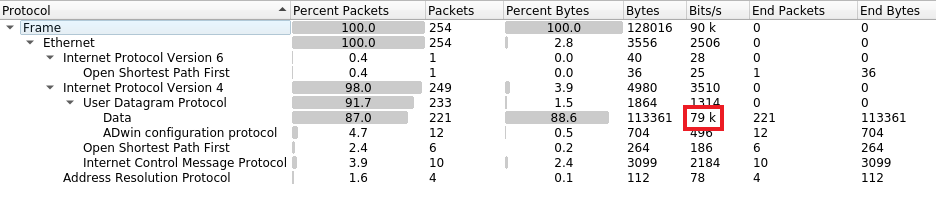
\includegraphics[width=.9\textwidth]{images/q5/unicast 1 cliente.png}}
    \caption{Cenário \textit{unicast} com 1 cliente}
\end{figure}

\begin{figure}[H]
    \centering
    \frame{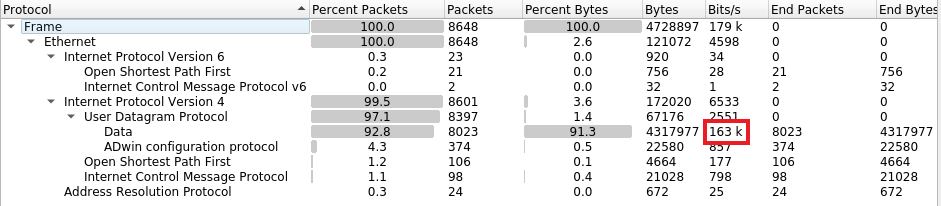
\includegraphics[width=.9\textwidth]{images/q5/unicast 3 clientes.png}}
    \caption{Cenário \textit{unicast} com 3 clientes}
\end{figure}

Já no cenário \textit{multicast}, o tráfego mantém-se, independentemente do número de clientes, permitindo às aplicações escalar, isto é, trabalhar com grandes números de clientes. Isto confirma-se nas figuras seguintes, onde se observa que o tráfego de pacotes relativos ao vídeo em streaming (MP4V-ES) mantém-se perto dos 100kbps, tanto sem clientes como com 3 clientes.

\begin{figure}[H]
    \centering
    \frame{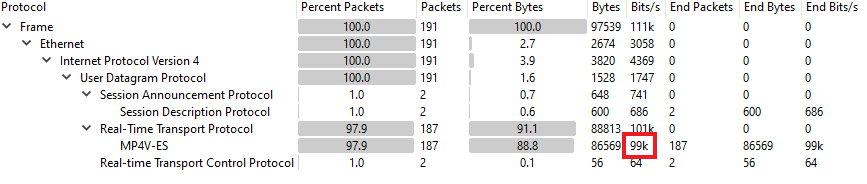
\includegraphics[width=.9\textwidth]{images/q5/multicast sem clientes.png}}
    \caption{Cenário \textit{multicast} sem clientes}
\end{figure}

\begin{figure}[H]
    \centering
    \frame{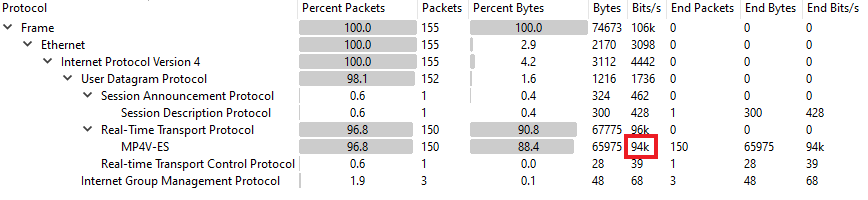
\includegraphics[width=.9\textwidth]{images/q5/multicast 3 clientes.png}}
    \caption{Cenário \textit{multicast} com 3 clientes}
\end{figure}

Assim, concluímos que o cenário \textit{multicast} é vantajoso para streaming com vários clientes, pois o tráfego na rede é constante, independentemente do número de clientes. Por esta mesma razão, este cenário pode ser desfavorável, caso estejam poucos ou nenhuns clientes conectados à stream.


%-------------------------- CONCLUSÃO --------------------------%
\clearpage
\section {Conclusões}

No âmbito deste trabalho prático abordamos o tema \textit{Streaming de áudio e vídeo a pedido e em tempo real} com o qual acreditamos ter cumprido todos os objetivos propostos pelos docentes da unidade curricular. 

Consideramos que este projeto teve especial relevo, na medida em que enriqueceu o nosso conhecimento na perceção da quantidade de largura de banda necessária para um \textit{streamer} receber um vídeo, correlacionar o ajuste de débitos de links com a resolução dos vídeos em \textit{streaming}, compreender as principais diferenças entre os cenários \textit{unicast} e \textit{multicast} focando, posteriormente, no cenário \textit{multicast} ao nível da rede, analisar, em termos de escalabilidade, o tráfego no \textit{link} de saída de um servidor com 1, 2 ou 3 clientes e aperfeiçoar as bases relativamente à forma como o \textit{DASH} funciona através de um ficheiro \textit{MPD}.

Em suma, o grupo considera que o propósito deste trabalho foi alcançado com sucesso, visto que intensificamos o nosso conhecimento sobre os temas em cima referidos.

%------------------------ BIBLIOGRAFIA ------------------------%
\clearpage
\begin{thebibliography}{}

\bibitem{livro}
Kurose, J., \& Ross, K. (2017). Computer Networking: A Top-Down Approach (7th ed.). Pearson.

\bibitem{q5}
\url{https://www.erg.abdn.ac.uk/users/gorry/course/intro-pages/uni-b-mcast.html}

\end{thebibliography}


\end{document}
